\documentclass{book}
\usepackage{graphicx}
\usepackage{amsmath}
\usepackage{float}
\usepackage{anyfontsize}
\usepackage[affil-it]{authblk}
\usepackage{fullpage}

\begin{document}

\author{Robert M. Johnson \\ rmj49@georgetotwn.edu}
\affil{ICBI \\ 2115 Wisconsin Ave NW, Suite 110}



\begin{titlepage}
\begin{center}

% Upper part of the page. The '~' is needed because \\
% only works if a paragraph has started.
{\fontsize{50}{150}\selectfont The medTurk Book}

\includegraphics[scale=0.7]{../ui/img/medkit.png}~  \\[1cm]
Aug 7, 2014
\end{center}
\end{titlepage}


\frontmatter


\chapter*{Preface}
ICBI at Georgetown University is proud to provide this simple, yet effective, tool for converting unstructured clinical notes into structured data for clinical research. This book contains instructions on what medTurk is, how to use it, and how to set it up.
\\
\\
- Robert M. Johnson (rmj49@georgetown.edu)

\tableofcontents

\mainmatter

\chapter{Introduction}

\section{What is medTurk?}
medTurk is web application that coordinates the ingenuity of humans to convert unstructured clinical notes into structured clinical data for research. medTurk assumes there are clinical research questions of interest that could be answered by reading patients' clinical notes. medTurk organizes these questions and their allowed answers, in what's called a Research Model (RM). RMs can can organize answers .

medTurk uses a Research Model (RM) to encapsulate the questions you want answered, allowable answers (i.e. control fields), and a 'trigger' that identfies phrases in clinical notes that probably contain the answer to the question sought.

To organize these questions and allowed answers, medTurk uses 'Research Models' or RMs for short. A RM is a simple JSON file that organizes questions, answers, and taxonomies.

medTurk allows multiple users at once to answer questions and the project status page reports the percantage of project complete. The following chapter guides the installation process. Chapter 3 gives instructions on how to setup your first project.


\chapter{Installation}
In this chaper we guide you through the process of setting up medTurk. medTurk depends on Python and several Python packages. In addition, it requires cTAKES for processing clinical notes, a local running instance of UMLS, and a local running instance of MongoDB. This chapter instructs you on how to setup each of these components. We begin with Python's dependencies.

\section{Python}
medTurk requires a Python version of at least 2.7.6. You can use following line in a Mac Terminal or Window's Command Line to retrieve the current Python version:
\begin{verbatim}
python --version
\end{verbatim}
Next, using pip, install the following Python packages:
\begin{verbatim}
pip install Flask
pip install mimerender
pip install pymongo
\end{verbatim}


\section{UMLS}
medTurk uses UMLS to look up names associated with CUIs reported by cTAKES. The following webpage provides instructions on how to setup a local UMLS MySQL database:

\begin{verbatim}
http://groups.csail.mit.edu/medg/projects/text/Load_UMLS_mysql.html
\end{verbatim}

Installation of this is necessary because medTurk always makes the assumption it is operated in a private, secure environment.

\section{cTAKES}
Install cTAKES by following the instructions provided here:

\begin{verbatim}
https://cwiki.apache.org/confluence/display/CTAKES/cTAKES+3.1+User+Install+Guide
\end{verbatim}





\section{mongoDB}
Finally, install mongoDB by following the instructions provided here:

\begin{verbatim}
http://www.mongodb.org/downloads
\end{verbatim}



\chapter{Research Models}
This section gives a detailed explanation of the research models (RMs) used in medTurk. Research models form the foundation of a research project and encapsulate the logic requiredto present the right information to workers to answer questions.

\section{How to Build a RM}
Unfortunately, medTurk to date does not provide a graphical user interface (GUI) to create a RM. Because of this, RMs must currently be created by hand or by programming. A RM in the end, is nothing more than a JSON (javascript object notation) file. For clarity, here we present a simple type of RM. One that investigates information on smoking and lung cancer:

\begin{verbatim}
{
  "name": "Investigation of Smoking and Lung Cancer",
  "children": [
    {
      "name": "Smoking",
      "question": "How many times has this patient smoked?",
      "answertype": "text",
      "triggers": [
        {
          "type": "keyword",
          "name": "smoke"
        },
        {
          "type": "keyword",
          "name": "cigarette"
        }
      ]
    },
    {
      "name": "Lung Cancer",
      "children": [
        {
          "name": "SCLC",
          "question": "Was this patient diagnosed with small cell lung cancer?",
          "answertype": "radio",
          "answers": [
            "yes",
            "no"
          ],
          "triggers": [
            {
              "type": "cui",
              "name": "?"
            }
          ]
        },
        {
          "name": "NSCLC",
          "question": "Was this patient diagnosed with non-small cell lung cancer?",
          "answertype": "radio",
          "answers": [
            "yes",
            "no"
          ],
          "triggers": [
            {
              "type": "cui",
              "name": "?"
            }
          ]
        }
      ]
    }
  ]
}
\end{verbatim}


At the root of this JSON, is the key \textbf{name}. This is where you name your research model. In this example, the name of the RM is \textbf{Investigation of Smoking and Lung Cancer}. 


The next key is \textbf{children}. Underneath this, is a list of either active nodes (ANs) or passive nodes (PNs). A passive node does not contain a question/answer, but instead, contains two key/value pairs:  "name" and "children". Passive nodes exist in order to categorize answers underneath. In our current example, the node named \textbf{Cancer} is a PN. If a worker answers \textbf{yes} in the AN named \textbf{Lung Cancer}, then that answer is automatically tagged with \textbf{Lung Cancer}. This allows downstream analysis for example, to group all patients that were diagnosed with lung cancer in general.

ANs contain the questions the workers will be asked. For each question, an answer type is specified under the key \textbf{answertype}. medTurk currently only answer types: \textbf{radio} and \textbf{text}. Choosing \textbf{text} means that a text box will appear for the worker to input text in. If radio type is chosen, then the key/value pair of "answers" must be present. Here, the value is a list of answers. In our current example, the AN of \textbf{Lung Cancer} has an answer radio type and has two possible answers: \textbf{yes} and \textbf{no}. Note that when choosing an \textbf{answertype} of \textbf{radio}, a worker may choose only one of the answers given in the list \textbf{answers}.

\section{Available Models}
Currently, medTurk contains only one research model that is used for extracting information on pediatric cancers, pediatric late effects, and pediatric cancer protocols. It is located in the following directory:

\begin{verbatim}
medturk/models/late_effects.json
\end{verbatim}




\chapter{Creating Your Own Project}

\section{Data Preparation}
medTurk requires patients' clinical notes to be in JSON format. Each JSON file should correspond to one patient. The name of the file is unimportant. Sample patient files can be viewed at:

\begin{verbatim}
https://github.com/ICBI/medkitpy/sample/patients/
\end{verbatim}

For convenience, we provide a snippet of one file here:
\begin{verbatim}
{
  "id": "1",
  "records": [
    {
      "id": "1_1",
      "date": "2000-5-15",
      "note": "Patient with newly diagnosed T-cell acute 
               lymphoblastic leukemia. Patient is being treated 
               according to COG protocol AALL0434 (On Study) 
               and is day X of Induction chemotherapy.
               Coming for follow-up and chemotherapy."
    },
    {
      "id": "1_2",
      "date": "2000-10-01",
      "note": "Patient with newly diagnosed T-cell acute
               lymphoblastic leukemia. Patient is being treated
               according to COG protocol AALL0434 Arm C (On Study)
               and is here today for follow-up and possible admission for
               Day x Consolidation chemotherapy (count dependent)."
    }
  ]
}
\end{verbatim}

As can be seen, at the top level, medTurk assumes two key/value pairs. The first key of \textbf{id} is the patient's unique identifier. The key \textbf{records} maps to an array of all records associated with that patient..

Each record requires three key/value pairs: \textbf{id}, \textbf{date}, and \textbf{note}.
\\
\\
\textbf{id} must be a unique record id across all patient records.
\\
\\
\textbf{date} assumes a YYY-MM-DD format. These dates are used when answer questions in order to arrange clinical notes across a time axis.
\\
\\
\textbf{note} contains the clinical note.


\subsection*{cTAKES}

Clinical notes must also be prepared for cTAKES processing. To do this, create a folder which contains two folders: 'input' and 'output'. In the input directory, each clinical note must be written as a .txt file. Using our previous the example, two text files would have to be generated:

\begin{verbatim}
1_1.txt
Patient with newly diagnosed T-cell acute lymphoblastic leukemia. 
Patient is being treated according to COG protocol AALL0434 
(On Study) and is day X of Induction chemotherapy. Coming for follow-up and chemotherapy.
\end{verbatim}

\begin{verbatim}
1_2.txt
Patient with newly diagnosed T-cell acute lymphoblastic leukemia. 
Patient is being treated according to COG protocol AALL0434 Arm C 
(On Study) and is here today for follow-up and possible admission 
for Day x Consolidation chemotherapy (count dependent).
\end{verbatim}


The name of the file must be in the format of \emph{recordId}.txt where \emph{recordId} is the recordId as found in the patients' JSON files. Thus, the file name is important here as medTurk uses this to map the processes clinical note back to its source.

\section{Running cTAKES}

In this section, we use cTAKES to process every clinical note contained the input folder described in the last section. To start up cTAKES, run the following command:

\begin{verbatim}
sh ./runctakesCPE.sh
\end{verbatim}

You should see something like the following:

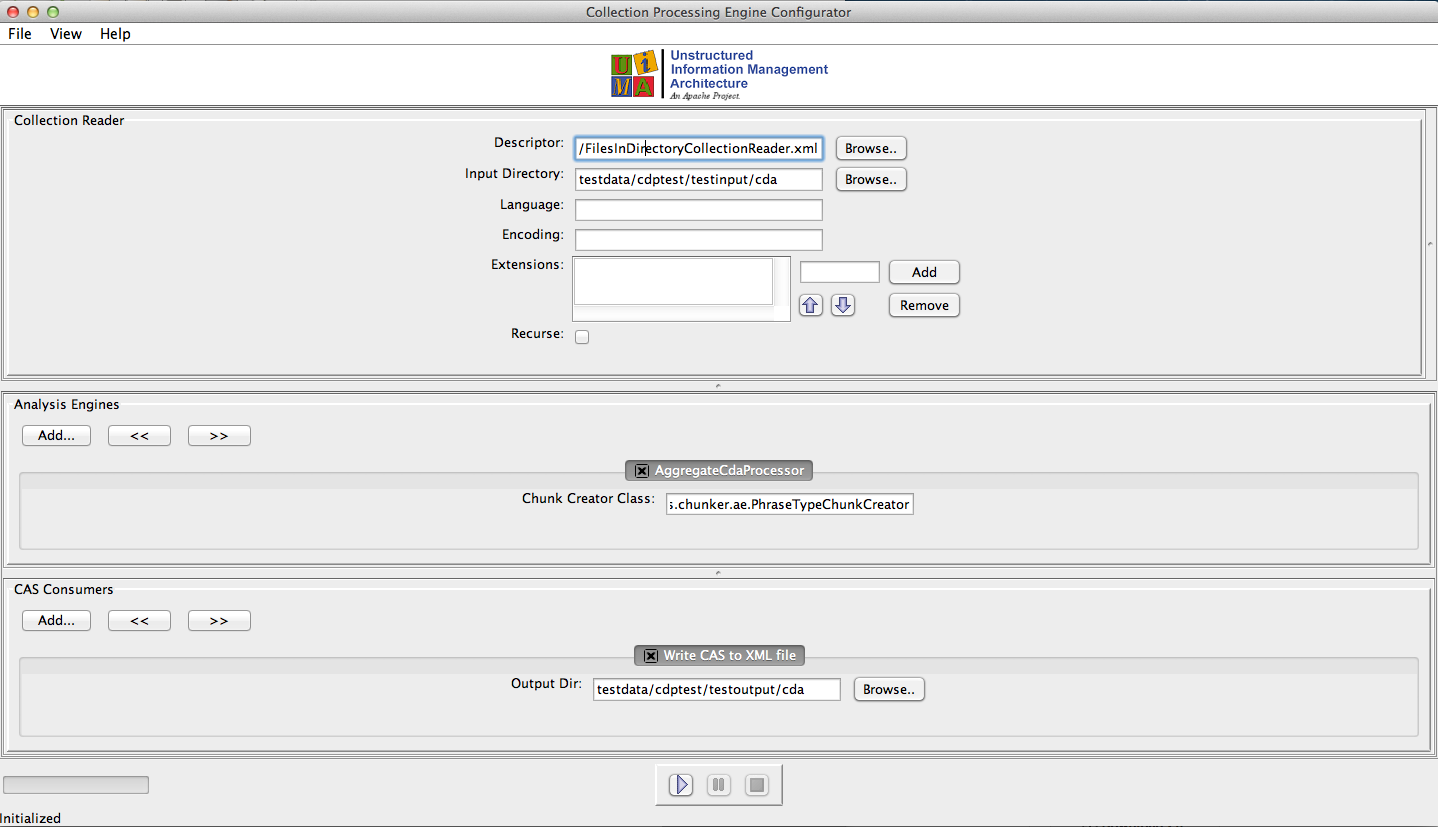
\includegraphics[scale=0.3]{ctakes.png}~  \\[1cm]

cTAKES provides instructions on how to batch process the files contained in the 'input' directory .
\\
medTurk uses cTAKES to process each clinical note for concepts and stores concepts according to three criteria.

\subsection*{Negation}
The first criteria is negation. The concept must have positive polarity, that is, it is not negated (e.g. the patient denies smoking).

\subsection*{Subject Analysis}
The second criteria is the concept must have a subject of patient. As an example, there are times when the a physician might write that a patient's father had lung cancer. In this example, the concept of "lung cancer" would have a subject of "Patient's Father". medTurk only extracts concepts which act directly on the patient.

\subsection*{Confidence}
The last criteria is confidence. cTAKES reports a confidence number for each extraction and medTurk only keeps concepts which have a confidence value of "1.0".



\section{Using medTurk}
To start up medTurk, ensure UMLS and MongoDB is running. Next, run the following script:

\begin{verbatim}
python run_server.py
\end{verbatim}
You should see something like the following:
\\
\\
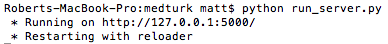
\includegraphics[scale=0.8]{run_server.png}~  \\[1cm]
Now, browse to the following URL in your browswer:

\begin{verbatim}
http://127.0.0.1:5000/medturk/index.html#/
\end{verbatim}

\subsection*{Home Page}
This is the landing page that contains a brief description of what medTurk is, and how to get started.

\subsection*{Create a Project Page}
To create a project, navigate to the project status page. You should see something like the following:

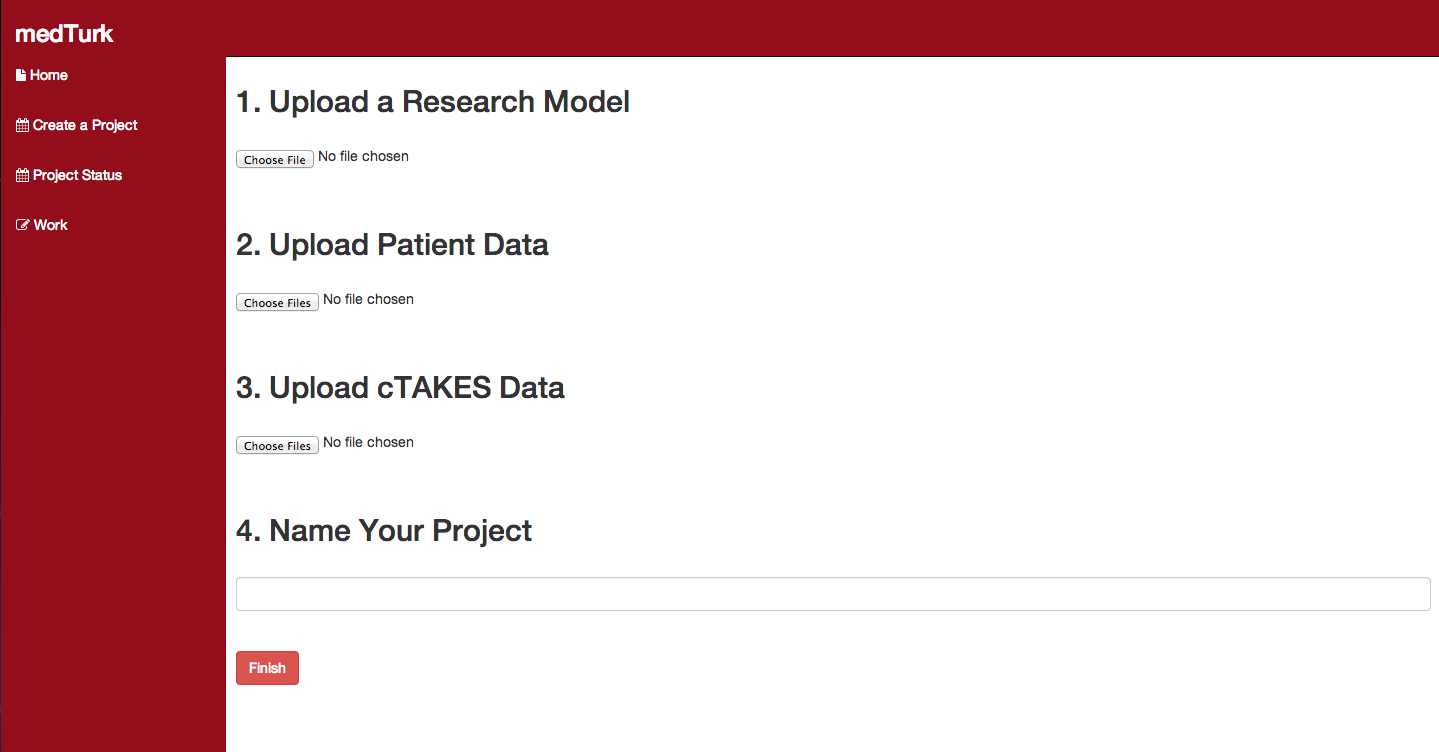
\includegraphics[scale=0.3]{create.png}~  \\[1cm]

\subsection*{Step 1}
Step 1 let's you upload your RM by navigating to it on your local computer. As an example, you may upload the late effects research model provided in medTurk found in:

\begin{verbatim}
medturk/models/late_effects.json
\end{verbatim}


\subsection*{Step 2}
Here, you can upload your one or more patient JSON files in the format explained in Section 3.1. As an example, you may upload the sample patient files found in:
\begin{verbatim}
medturk/example/patients/
\end{verbatim}


\subsection*{Step 3}
The Step 2, allows you to upload the processed cTAKES files. An an example, you may upload the sample cTAKES files found in:
\begin{verbatim}
medturk/example/ctakes/output/
\end{verbatim}

\subsection*{Step 4}
Here you may pick a name for your project. Click Finish and the project will be created.
\\
\section{Navigating medTurk}
In addition to the \textbf{Home} and \textbf{Create a Project Page} already mentioned,  medTurk includes two additional pages.

\subsection*{Project Status Page}
You may visualize the research model and view the percentage of project completion in the 'Project Status' page. This page also allows you to download answered questions in CSV format. This file can then be used for statistical analysis. 


\subsection*{Work Page}
You many answer questions by visiting this page. Each question provides clinical notes that are relevant to answering the question. 



\end{document}             % End of document.